%%%%%%%%%%%%%%%%%%%%%%%%%%%%%%%%%%%%%%%%%%%%%%%%%%%%%%%%%%%%%%%%%%%%%%%%%%%%%%%%%%%
% Team: Rainy
% Members: Rain  Dickson  Sareddy
% Relative files:
% Note: Do not compile this file compile Main.tex to get the pdf file instead.
%%%%%%%%%%%%%%%%%%%%%%%%%%%%%%%%%%%%%%%%%%%%%%%%%%%%%%%%%%%%%%%%%%%%%%%%%%%%%%%%%%%
\subsection{Latent Semantic Analysis}
Latent Semantic Analysis is a kind of Corpus-Based similarity anaysis. Corpus-Based similarity is a semantic similarity measure which determines the similarity between the words based on the information gained from corpora. A Corpus is a large collection of texts and it is used for language research. Latent Semantic Analysis(LSA) assumesthat the words with close meaning will mostly occur inthe similar group. A matrix which contains word counts per paragraph was constructed from a  dataset.In order to reduce the number of columns, singular ue decomposition (SVD) is used and it preserves the similarity structure among the rows. The LSA approach is extended by focusing on term vectors instead of the representation of dual document-term and cosine measures between the vectors are expressed based on the semantic relatedness between two texts.
 
\subsection{Metadata Extraction}
Metadata Extractor is the module which can extract metadata in PDF files such as title, subheading, doi, etc. We use python package pyPdf to extract metadata directly and use metadata to do a couple of things. First, we extract titles of articles returning those to the web page as search results. Second, we use metadata extractor to extract subheadings which are treated as the definition of break point to split PDF file i.e. one article will be separated into small pieces based on subheading. The small pieces will convert into .txt files by the .txt converter we built so that we can take .txt files into similarity comparison and get the most relative parts in the article. Third, we extract doi from the article. 

 \subsection{Text Processing}
 After converting an article from .pdf file format to .txt format, we read the converted text file to the program and do preprocessing task. First, delete all stopwords(ex. is am are the etc) that are irrelavent to the article. Second, remove all punctuation and any non-alphabet characters  in the article. Third, tokenize the article into words and count the frequency of each word appeared in the article. Finally, remove the word only appeared once in the article because low ocurrance indicates less importance of the word to the article.


\subsection{Similarity Comparison}
	\begin{figure*}[htb]
		\begin{center}
			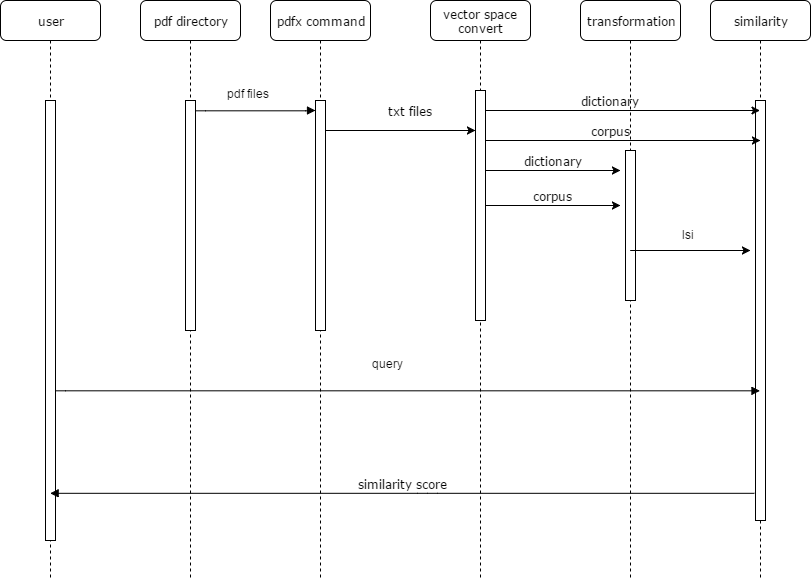
\includegraphics[width=0.8\textwidth]{Rainy_Sequence_diagram}
		\end{center}
		\caption{Sequence diagram of text similarity compare functionality.\label{Sequence diagram}}
	\end{figure*}
\newpage